\section{Reactor like TGE-model}\label{sec:thunderstorm/reactor}

Общим недостатком рассмотренных выше моделей является упрощенная модель электрического поля: оно считается однородным по величине и направлению, что очевидно не так и в полу должны присутствовать разного рода неоднородности, вызванные как краевыми эффектами, так и возникновением сложных конфигураций зарядов. Точное моделирование и анализ динамики лавин убегающих электронов представляет собой сложную задачу, поэтому рассмотрим упрощенную модель что бы оценить потенциальные результаты, которые могут принести исследования в данном направлении. 

Чем ситуация в неоднородном по направлению поле отличается от развития лавин в однородном поле? Когда поле однородно то если гамма-кванты рождают новые затравочные электроны, то лавины от этих электронов будут направлены в том же направлении что и  первая лавина, но при этом их вершина будет смещена к  краю облака, что будет постепенно приводить к затуханию (как показано в предыдущих главах). Если же поле неоднородно по направлению, то направление новых лавин зависит от локальной конфигурации поля и таким образом может возникнуть ситуация изображенная на рисунке --- гамма-кванты от первичной лавины "зажигают" новые локальные ускоряющие ячейки, которые генерирует гамма кванты с угловым распределение значительно развернутым относительно углового распределения исходной лавины, что способствует более равномерному распределению новых затравочных электронов по облаку и как следствие  самоподдерживающей генерации лавин убегающих электронов.
Что бы смоделировать этот процесс, мы рассмотрим такую модель:
\begin{itemize}
    \item Используем только один изменяемый параметр --- локальный коэффициент размножения гамма-квантов, который дает обобщенное описание состояние атмосферы (величины электрического поля, плотности воздуха, вероятности зажигания ячейки и. т. д.)
    \item  Пренебрежем значением энергии гамма-квантов, пробег гамма-квантов будем разыгрывать на основе экспоненциального распределения с фиксированной длинной свободного пробега, много меньшей размеров облака;
    \item Также мы будем считать что при взаимодействии он гарантированно зажигает ячейку (фактически вероятность зажечь ячейку мы спрятали в локальном коэффициенте размножения);
    \item При зажигании ячейки мы не моделируем прохождение электронной лавины, а сразу генерируем вторичные гамма-кванты, их количество разыгрывается с помощью распределения Пуассона с локальным коэффициентом размножения гамма-квантов в качестве среднего, направление движения рожденных гамма-квантов считается однонаправленным с направлением электрического поля в точке рождения;
    \item Электрическое поле генерируются случайным образом на основе положения электрических зарядов местоположения которых разыграны на основе гауссова случайного блуждания;
    \item Облако представляется в виде куба со стороной в один километр, частицы покинувшие облако перестают отслеживаться.
\end{itemize}

В результате моделирования можно выделить три сценария: 
\begin{itemize}
    \item При малых значения локального коэффициента размножения роста гамма-квантов не происходит и высокоэнергетические процессы быстро затухают;
    \item При локальном коэффициенте размножения равным примерно 1.7 становится возможным медленное нарастание числа гамма-квантов, которое приводит к относительно стабильному самоподдерживающийся процессу, который однако с течением времени все же затухает. В целом этот сценарий хорошо описывает TGE-подобные явления;
    \item При превышении локальным коэффициентом размножения значения 1.8 происходит взрывной экспоненциальный рост числа гамма-квантов. Быстрый рост и большое количество гамма-квантов позволяет сказать что этот сценарий хорошо описывают TGF-подобные явления.
\end{itemize}

Для того чтобы проиллюстрировать эти три сценария, в работе приведены графики роста числа гамма-квантов в облаке от времени. Так график показывает затухание процессов при недостаточном значении локального коэффициента размножения, в данном примере несмотря на то что начальные гамма-кванты смогли сгенерировать некоторое количество вторичных частиц за время порядка 300 микросекунд все процессы затухли. График напротив показывает экспоненциальный рост за времена порядка 50-100 микросекунд (следует отметить что это согласуется со временем реально наблюдаемых TGF) при значения локального коэффициента размножения большего 1.8. Очень интересен график в нем наблюдается постепенный рост на достаточно большом (порядка 3 секунд) времени, что позволяет нам перейти от действующий на микровременных масштабах TGF к долговременным TGE. 

\begin{figure}
    \centering
    \begin{overpic}[scale=.5]{thunderstorm/rltge/electric_streams.pdf}
        \put(15,53){\includegraphics[scale=.015]{thunderstorm/rltge/cell.pdf}}
        \put(20,69){\text{Ускоряющая ячейка}}
        \put(10,10){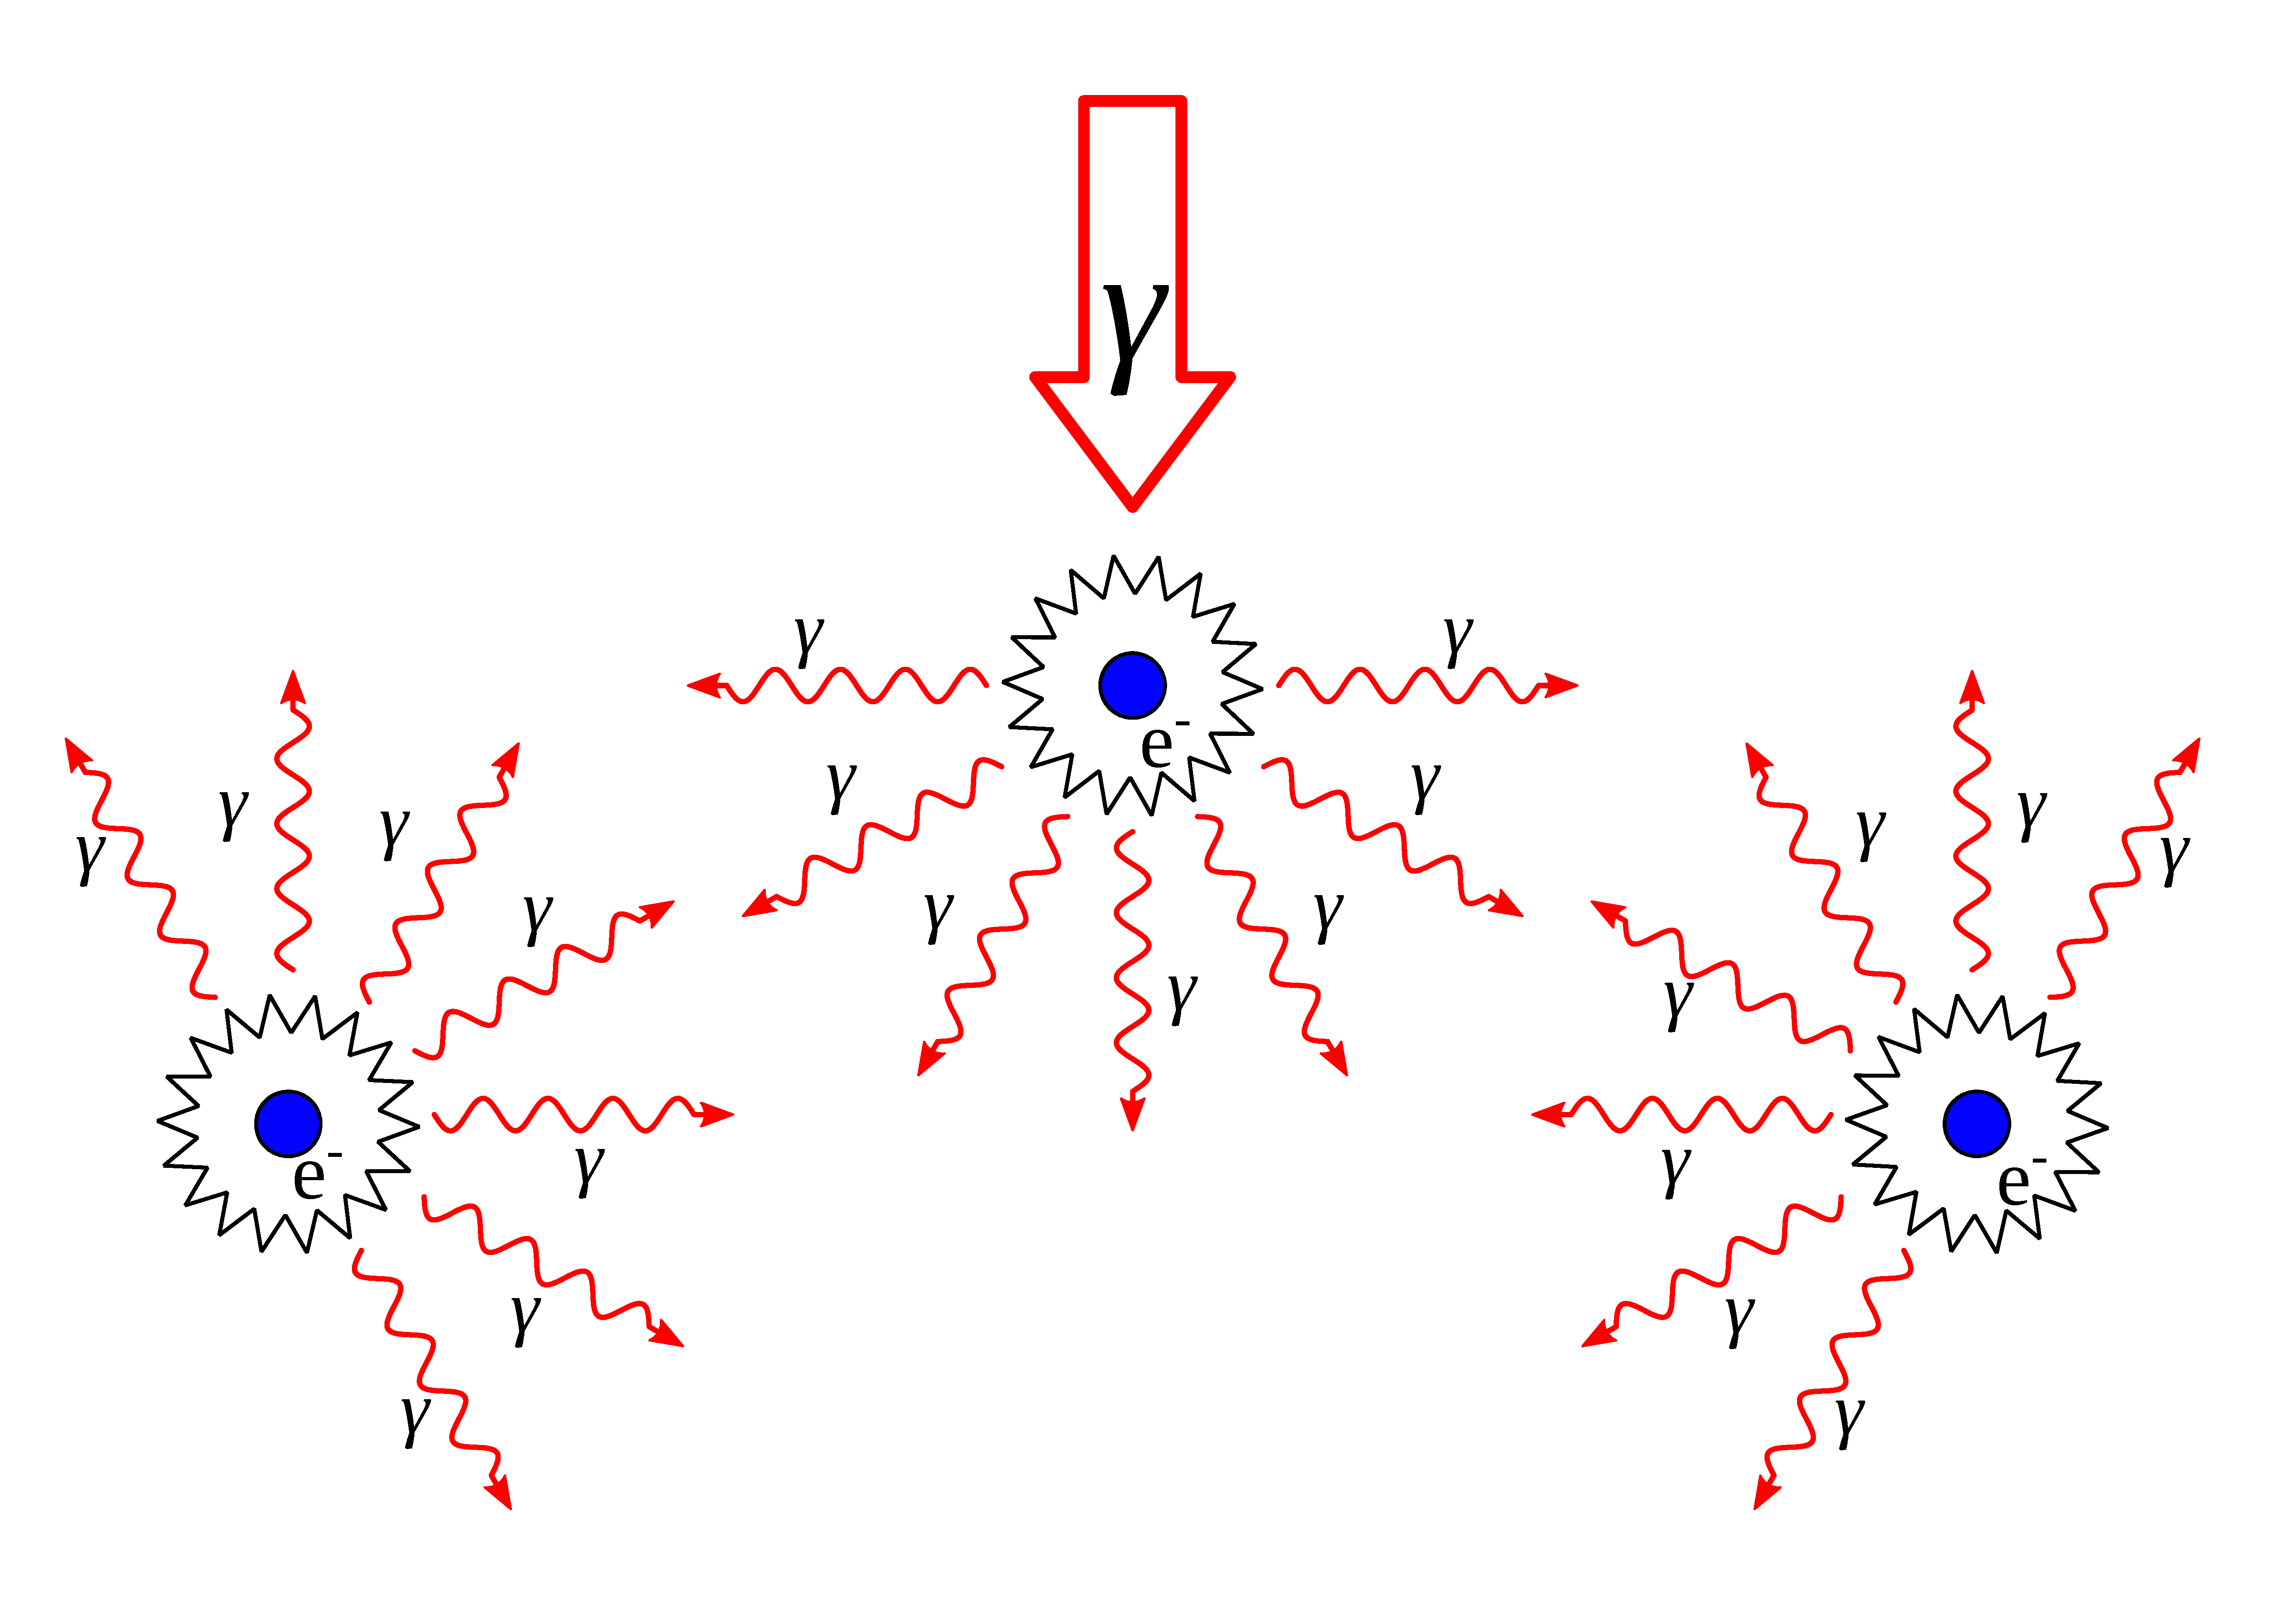
\includegraphics[scale=.15]{thunderstorm/rltge/draw.pdf}}
    \end{overpic}
    \caption{
        Processes occurring in the RL-TGE model: gamma quanta run local acceleration processes in different parts of the cloud with a multidirectional electric field.
    }
    \label{fig:rl}
\end{figure}


\begin{figure}[t]
    \begin{center}
        \begin{minipage}[h]{0.49\linewidth}
            \center{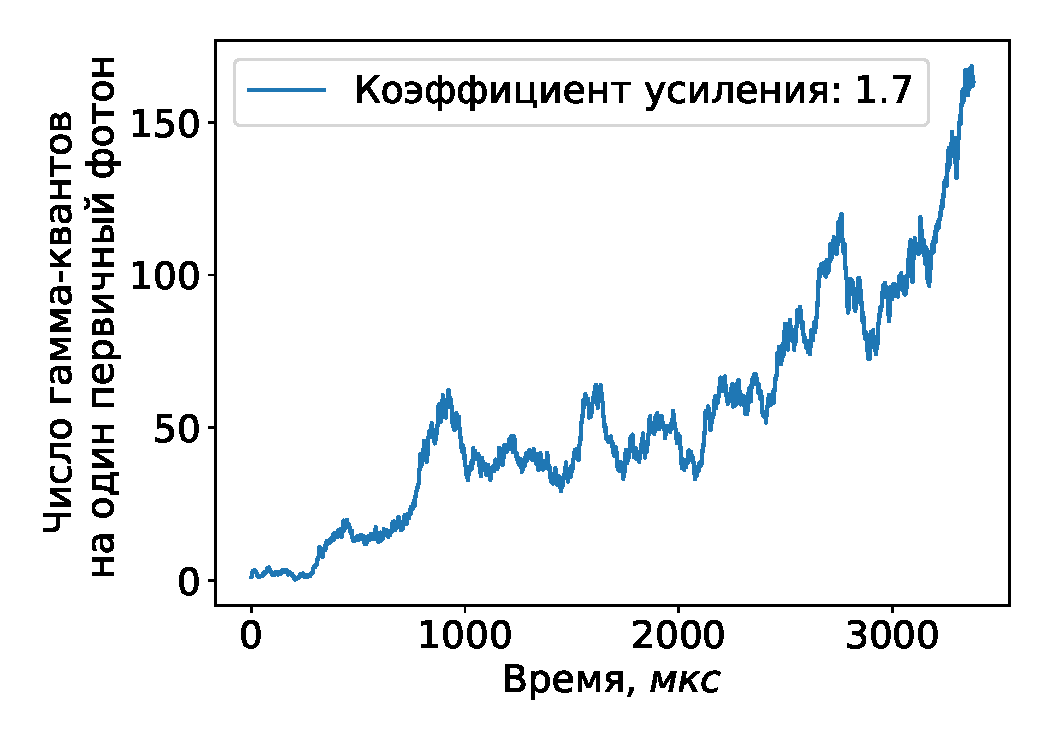
\includegraphics[width=\linewidth]{thunderstorm/RL_proofTGE.pdf} \\ а)}
        \end{minipage}
        \hfill
        \begin{minipage}[h]{0.49\linewidth}
            \center{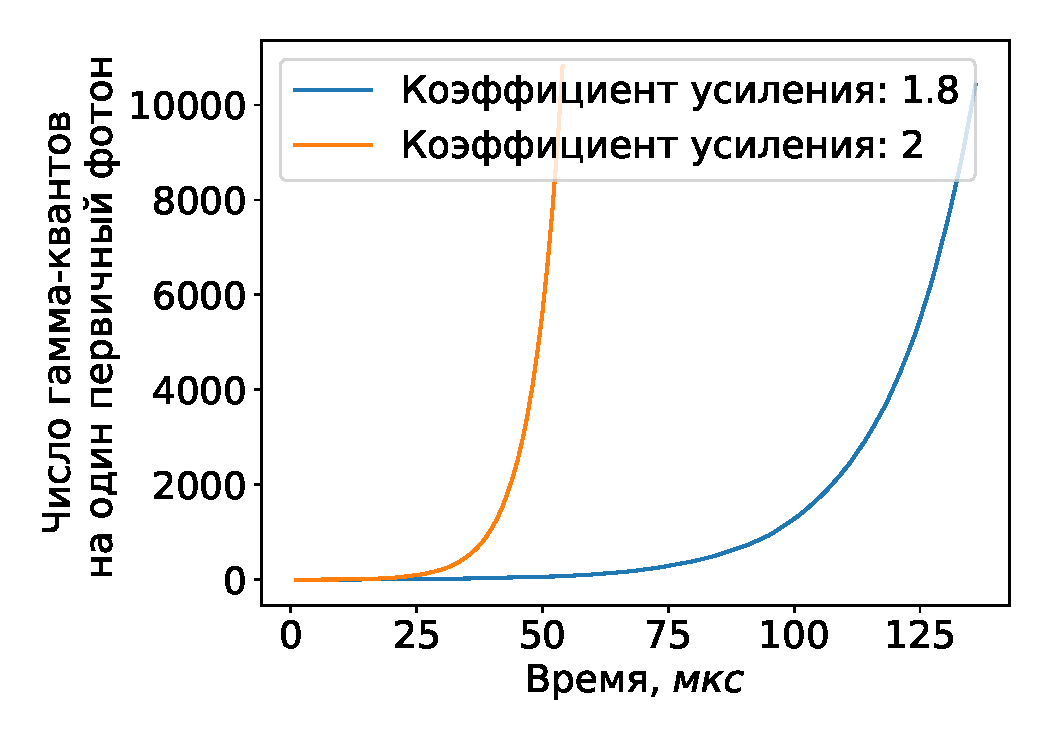
\includegraphics[width=\linewidth]{thunderstorm/RL_proofTGF.pdf}   \\ б)}
        \end{minipage}
        \caption{а) TGE-подобное нарастание. б) TGF-подобное нарастание.}
    \end{center}
    \label{thunder:rl_1}
\end{figure}


\begin{figure}[t]
    \begin{center}
        \begin{minipage}[h]{0.49\linewidth}
            \center{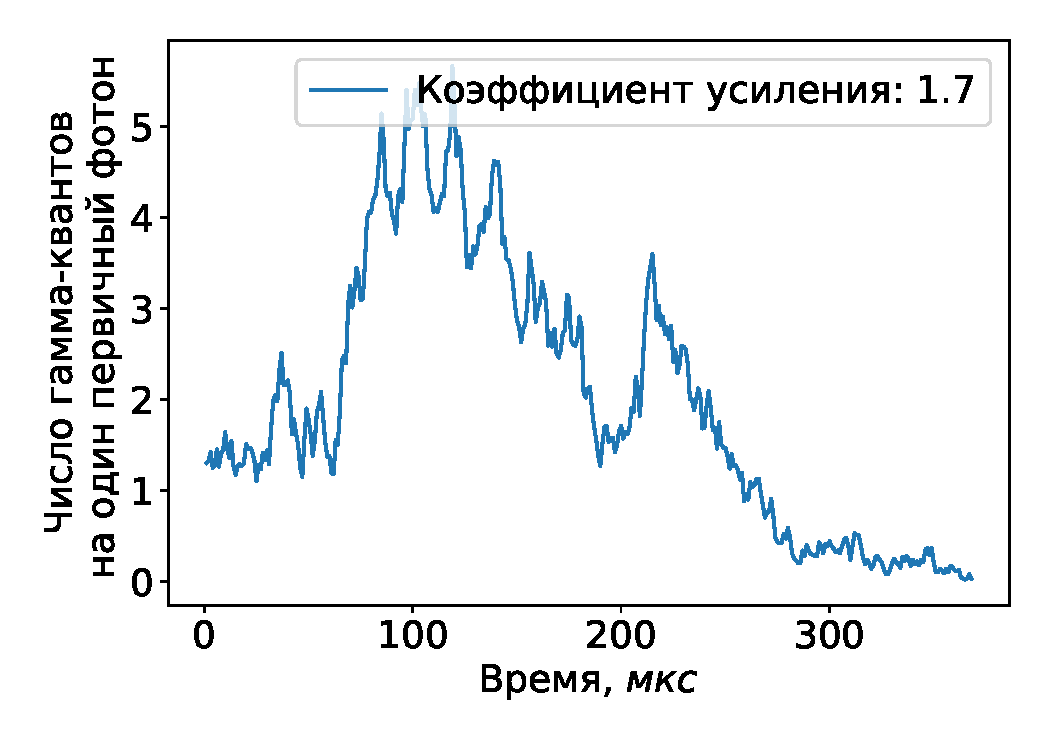
\includegraphics[width=\linewidth]{thunderstorm/RL_Extinction.pdf} \\ а)}
        \end{minipage}
        \hfill
        \begin{minipage}[h]{0.49\linewidth}
            \center{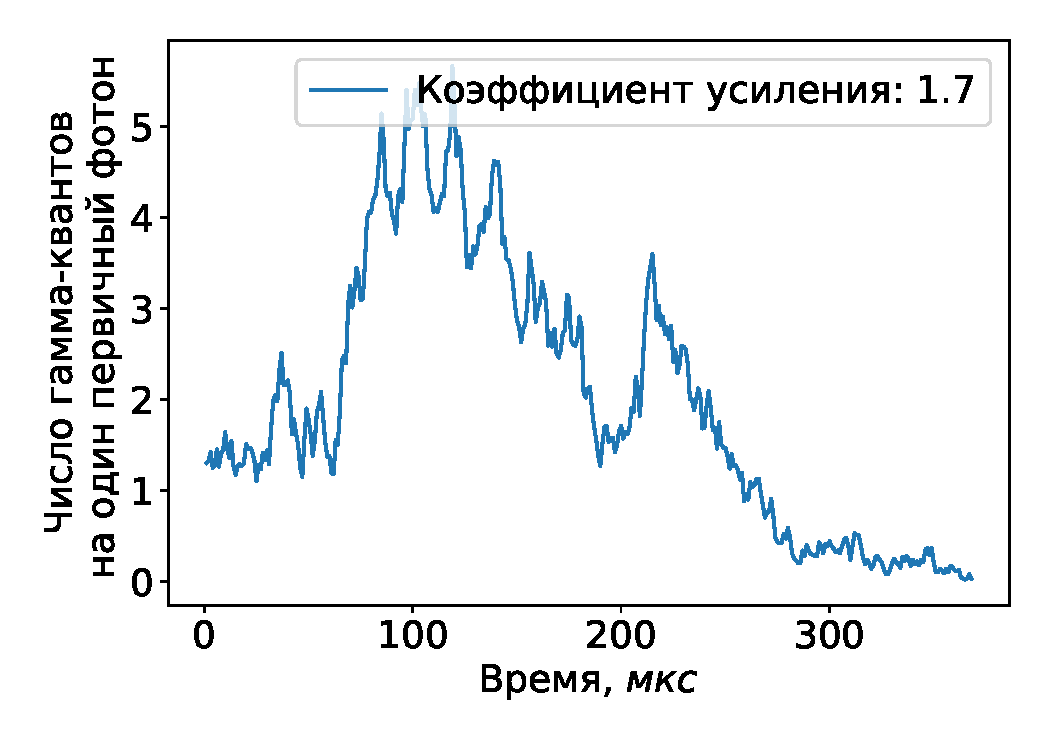
\includegraphics[width=\linewidth]{thunderstorm/RL_Extinction.pdf}   \\ б)}
        \end{minipage}
        \caption{а) Затухание лавины. б) placeholder.}
    \end{center}
    \label{thunder:rl_2}
\end{figure}

Характер высокоэнергичных процессов в облаке в нашей модели напоминает происходящее в ядерных реакторах, где изменение одного параметра (коэффициента размножения нейтронов приводит либо к затуханию реактора, либо к стабильной выработке энергии, либо к взрыву топлива), поэтому мы называем нашу модель атмосферным реактором, и так же по аналогии можем выделить подкритический и критический режим работы реактора. Критический режим соответствует активному размножению гамма-квантов, которые порождают все больше лавин убегающих электронов что приводит к активной ионизации объема облака. Подкритический режим соответствует значению коэффициента размножения  при котором с одной стороны процессы в облаке постоянно стартуют в следствии подпитки внешними КЛ и затухают в следствии малости коэффициента размножения, с другой стороны  близкому к достаточному для начала работы в критическом режиме. Как показывает наше моделирование небольшое изменение локального коэффициента размножения позволяет перейти из подкритического режима в критический, что открывает для нас интересные возможности. Так облако можно представить как саморегулирующуюся системы в которой в следствии накопления заряда и роста электрического поля растет коэффициент размножения, что приводит к росту ионизации, что может приводить к появлению микроразрядов на гидрометеорах, что уменьшает коэффициент размножения и препятствует дальнейшей разрядке облака. Или например можно описать столкновение двух облаков, которые будучи в подкритическом режиме при столкновении переходят в критический режим. В целом проведенное моделирование хоть и носит очень приближенный характер, дает нам представление о перспективах модели со сложным полем по сравнению с более простыми моделями в которых рассматривается только однородное поле. Реакторная модель позволяет описывать рождение TGF и TGE в зависимости от состояние в облаке, внутриреакторные потоки гамма-квантов позволяют описать избыток нейтронов наблюдающийся в работе (ссылка на гуревича). Результаты моделирования изложен в статье, исходный код доступен по ссылке.
